\documentclass[10pt]{article}
\usepackage[utf8]{inputenc}
\usepackage{parskip}
\usepackage[margin = 1in]{geometry}
\usepackage{xcolor}
\usepackage[colorlinks = true,linkcolor = blue, urlcolor  = blue,citecolor = blue,anchorcolor = blue]{hyperref}
\usepackage{framed}
\usepackage{apacite}
\usepackage[authoryear,sort]{natbib}
\usepackage{amsmath}
\usepackage{amssymb}
\bibliographystyle{apalike}
\newcommand{\E}{\textrm{E}}
\renewcommand*{\theenumi}{\thesection.\arabic{enumi}}
\renewcommand{\P}{\text{P}}
\usepackage{tikz}
\usetikzlibrary{arrows,shapes.arrows,positioning,shapes,patterns,calc}

\begin{document}

\begin{Large} 
Info 6751. Fall 2022. Problem Set 8. Due on Canvas by 5pm on 24 Oct.
\end{Large}
\hline \vskip .1in

Submit a PDF. For Part 2, either embed your code in the PDF or include as an attachment.

\section{Causal identification in dynamic settings (30 points)}

In each DAG below, the researcher observes the outcome $Y$ and the variables $\{\vec{L}_t,A_t\}$ for every time period $t$. The researcher does not observe $U$.

\begin{tikzpicture}
    \node[anchor = north west] at (-.5,2) {Setting A)};
    \node (a0) at (0,0) {$A_0$};
    \node (a1) at (1,0) {$A_1$};
    \node (y) at (2,0) {$Y$};
    \draw[->, thick] (a0) to[bend left = 45] (y);
    \draw[->, thick] (a1) -- (y);
    \draw[->, thick] (a0) -- (a1);
    \node at (0,-2.2) {};
\end{tikzpicture}
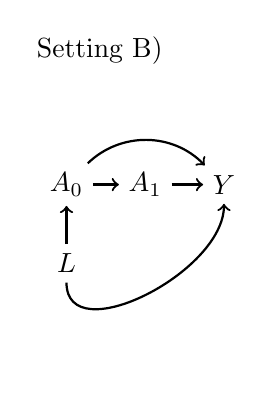
\begin{tikzpicture}
    \node[anchor = north west] at (-.5,2) {Setting B)};
    \node (l0) at (0,-1) {$L$};
    \node (a0) at (0,0) {$A_0$};
    \node (a1) at (1,0) {$A_1$};
    \node (y) at (2,0) {$Y$};
    \draw[->, thick] (a0) to[bend left = 45] (y);
    \draw[->, thick] (a1) -- (y);
    \draw[->, thick] (a0) -- (a1);
    \draw[->, thick] (l0) -- (a0);
    \draw[->, thick] (l0) to[out = 270, in = 270] (y);
    \node at (0,-2.2) {};
\end{tikzpicture}
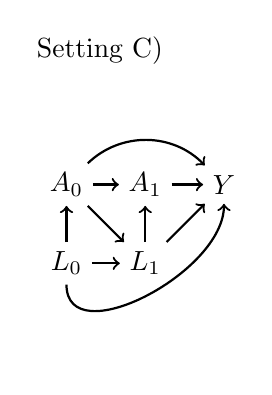
\begin{tikzpicture}
    \node[anchor = north west] at (-.5,2) {Setting C)};
    \node (l0) at (0,-1) {$L_0$};
    \node (a0) at (0,0) {$A_0$};
    \node (l1) at (1,-1) {$L_1$};
    \node (a1) at (1,0) {$A_1$};
    \node (y) at (2,0) {$Y$};
    \draw[->, thick] (a0) to[bend left = 45] (y);
    \draw[->, thick] (a1) -- (y);
    \draw[->, thick] (a0) -- (a1);
    \draw[->, thick] (a0) -- (l1);
    \draw[->, thick] (l0) -- (a0);
    \draw[->, thick] (l1) -- (a1);
    \draw[->, thick] (l0) -- (l1);
    \draw[->, thick] (l0) to[out = 270, in = 270] (y);
    \draw[->, thick] (l1) -- (y);
    \node at (0,-2.2) {};
\end{tikzpicture}
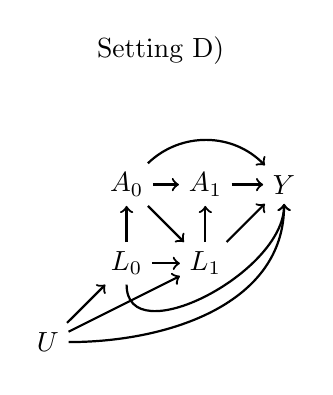
\begin{tikzpicture}
    \node[anchor = north west] at (-.5,2) {Setting D)};
    \node (u) at (-1,-2) {$U$};
    \node (l0) at (0,-1) {$L_0$};
    \node (a0) at (0,0) {$A_0$};
    \node (l1) at (1,-1) {$L_1$};
    \node (a1) at (1,0) {$A_1$};
    \node (y) at (2,0) {$Y$};
    \draw[->, thick] (a0) to[bend left = 45] (y);
    \draw[->, thick] (a1) -- (y);
    \draw[->, thick] (a0) -- (a1);
    \draw[->, thick] (a0) -- (l1);
    \draw[->, thick] (l0) -- (a0);
    \draw[->, thick] (l1) -- (a1);
    \draw[->, thick] (l0) -- (l1);
    \draw[->, thick] (l0) to[out = 270, in = 270] (y);
    \draw[->, thick] (l1) -- (y);
    \draw[->, thick] (u) -- (l0);
    \draw[->, thick] (u) -- (l1);
    \draw[->, thick] (u) to[out = 0, in = 270] (y);
    \node at (0,-2.2) {};
\end{tikzpicture}
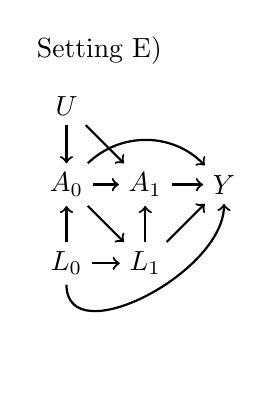
\begin{tikzpicture}
    \node[anchor = north west] at (-.5,2) {Setting E)};
    \node (u) at (0,1) {$U$};
    \node (l0) at (0,-1) {$L_0$};
    \node (a0) at (0,0) {$A_0$};
    \node (l1) at (1,-1) {$L_1$};
    \node (a1) at (1,0) {$A_1$};
    \node (y) at (2,0) {$Y$};
    \draw[->, thick] (a0) to[bend left = 45] (y);
    \draw[->, thick] (a1) -- (y);
    \draw[->, thick] (a0) -- (a1);
    \draw[->, thick] (a0) -- (l1);
    \draw[->, thick] (l0) -- (a0);
    \draw[->, thick] (l1) -- (a1);
    \draw[->, thick] (l0) -- (l1);
    \draw[->, thick] (l0) to[out = 270, in = 270] (y);
    \draw[->, thick] (l1) -- (y);
    \draw[->, thick] (u) -- (a0);
    \draw[->, thick] (u) -- (a1);
    \node at (0,-2.2) {};
\end{tikzpicture}

The researcher wants to know the expected potential outcome $\E(Y^{a_0,a_1})$ under an intervention to set $A_0 = a_0$ and $A_1 = a_1$. In which of settings A--E can this causal estimand be identified using
\begin{enumerate}
    \item (10 points) The simple mean $\E(Y\mid A_0 = a_0, A_1 = a_1)$
    \item (10 points) Inverse probability weights applied in a marginal structural model, adjusting at each period for the observed past
\end{enumerate}

Now focus on Setting D.
\begin{enumerate}
    \item[1.3.] (10 points) For Setting D, explain how $L_1$ complicates the quest to jointly identify the causal effects of $A_0$ and $A_1$ using our usual adjustment strategies.
\end{enumerate}

\section{Causal estimation in a dynamic setting (20 points)}

This problem is an extension of the class exercise from Tuesday. The goal is for you to practice estimating a marginal structural model in a dynamic setting designed to be as simple as possible.

Suppose a teacher observes students who are struggling academically ($L_t = 1$) or not ($L_t = 0)$ in every time period $t$. The teacher can assign students to receive extra support ($A_t = 1$) or not ($A_t = 0$). The outcome $Y$ is a subsequent measure of skills (e.g., can the student read a picture book to the teacher). The attached \texttt{pset8.csv} contains a simulated setting with $n = 128$ students. It is not identical to the one from class, but as in class:
\begin{itemize}
    \item Treatment $A_t = 1$ is assigned with higher probabilities to students who are struggling $L_t = 0$.
    \item Students who are treated in one period $A_0 = 1$ are never struggling in the next period $L_1 = 0$.
\end{itemize}
Assume the causal structure represented by Setting D above. Using these data,
\begin{enumerate}
    \item (3 points) Fit a logistic regression for each $A_t$, including as predictors all pre-treatment variables entered without interactions.
    \item (3 points) Predict the probability of $A_t = 1$ at each time period for every unit. Remember that in R you will need the \texttt{type = "response"} option. For grading, what is the predicted value of $A_0$ for the first unit in the sample?
    \item (3 points) Define the generalized propensity score $\pi_{it}$ at each time period $t$ for each unit $i$. When $A_{it} = 1$ this will be the number from 2.2. When $A_{it} = 0$, it will be $1 - (\texttt{that number})$.
    \item (3 points) Define a weight for each unit: $w_i = \frac{1}{\pi_{i0}}\frac{1}{\pi_{i1}}$. For grading, what is the weight on the first unit in the sample?
    \item (3 points) Estimate a marginal structural model of the form $\E(Y^{a_0,a_1}) = \alpha + \beta_0 a_0 + \beta_1 a_1$. Report the coefficients.
    \item (5 points) What does your model estimate for the average causal effect $\E(Y^{1,1} - Y^{0,0})$?
\end{enumerate}

\end{document}

